\documentclass[8pt]{beamer}

\usetheme[progressbar=frametitle]{metropolis}
\usepackage{booktabs}
\usepackage[scale=2]{ccicons}
\usepackage{ragged2e}
\usepackage{pgfplots}
\usepgfplotslibrary{dateplot}
\usepackage{xspace}
\newcommand{\themename}{\textbf{\textsc{metropolis}}\xspace}

\title{\textbf{CMS at LHC}}

\date{\today}
\author{\textbf{Diego Barón}}
\institute{Universidad de Antioquia, Instutito de Física.}

\begin{document}

\maketitle

\begin{frame}{Table of contents}
  \setbeamertemplate{section in toc}[sections numbered]
  \tableofcontents[hideallsubsections]
\end{frame}


\section{Motivation.}

\begin{frame}[fragile]{Motivation}

Particle physics experiments can be made studying cosmic rays, solar neutrinos, dark matter in galaxies, etc. 

\begin{exampleblock}{But don't forget accelerators... }
This experiments are the most popular because we can control almost all the initial conditions:
\begin{itemize}
\item The particles involved.
\item The energy of the beams.
\item The geometry of the experiment
\item The amount of particles. 
\end{itemize}    
\end{exampleblock}

Experimental particle physicists must know and understand how experiments works in order to know:
\begin{itemize}
\item What to look for.
\item And how to.
\end{itemize}

\end{frame}

\section{The problem.}
\begin{frame}[fragile]{The problem.}
\centering
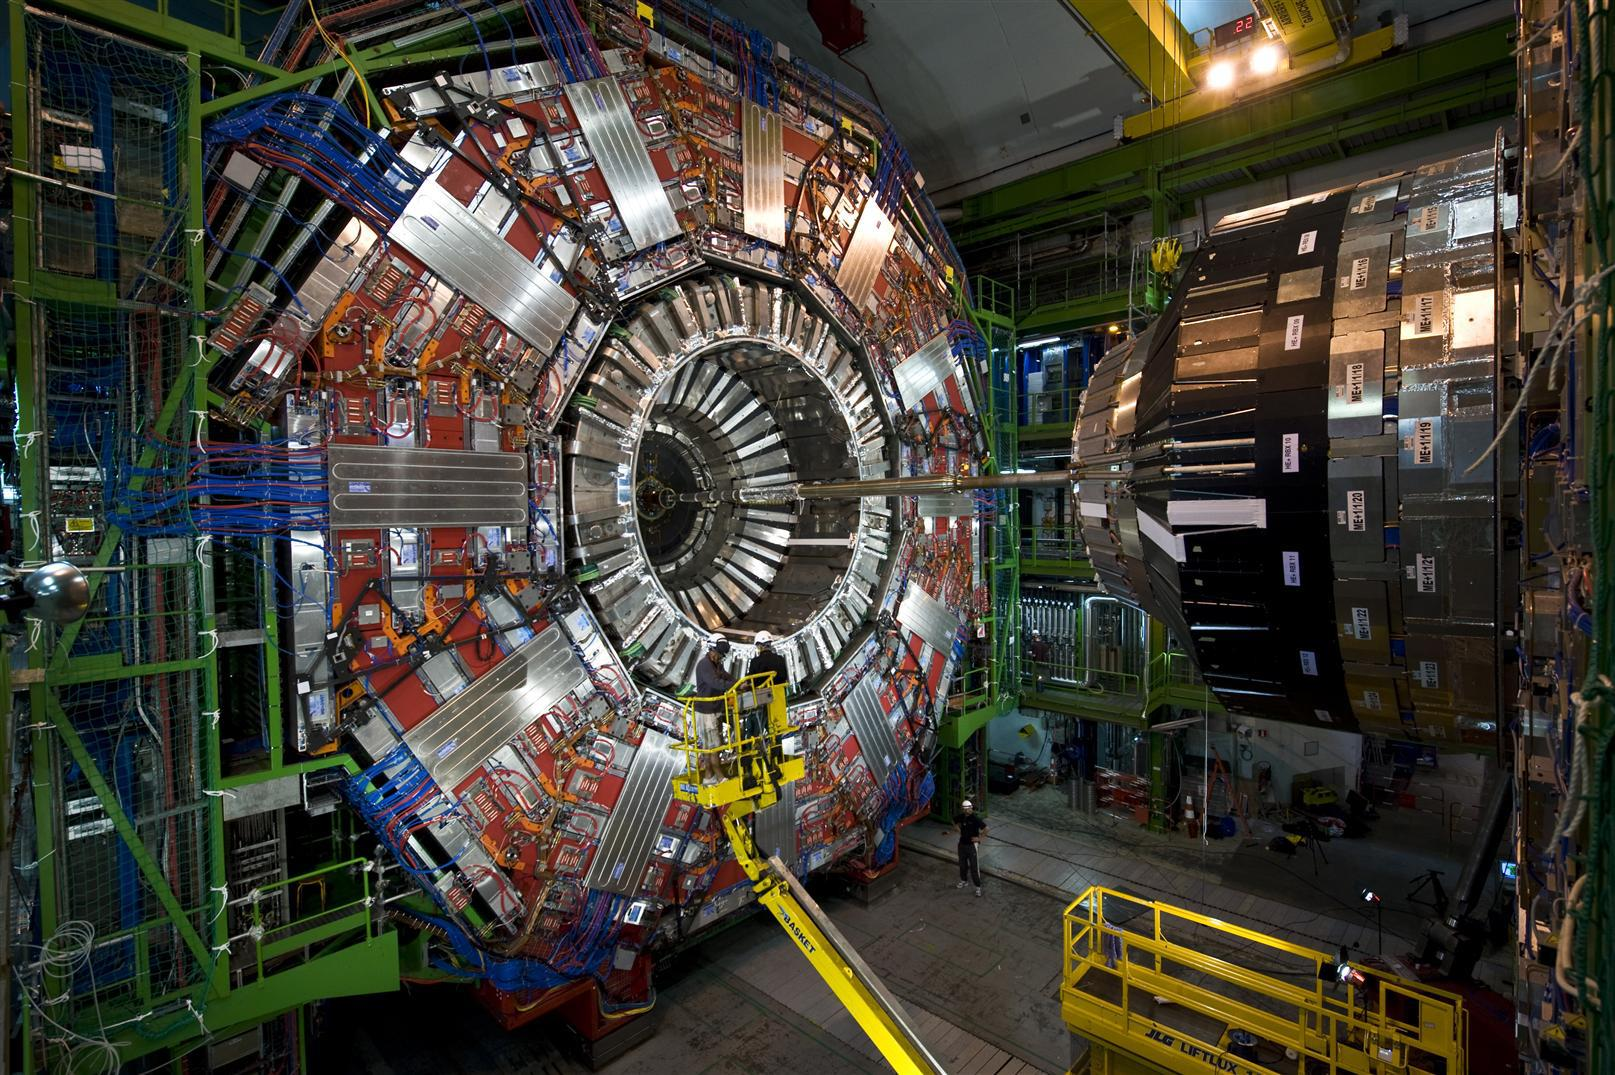
\includegraphics[height=7cm,width=9cm]{1}
\metroset{block=fill}
\begin{exampleblock}{\centering The question is...}
\centering
¿How does CMS at LHC works?

\end{exampleblock}


\end{frame}

\section{First LHC.}

% HHHHHHHHHHHHHHHHHHHHHHHHHHHHHHHHHHHHHHHHHHHHHHHHHHHHHHHHHHHHHHHHH

\begin{frame}[fragile]{LHC.}
Is the main accelerator managed by CERN (European Organization for Nuclear Research). 
21 member states-113 participant countries.

It`s the biggest particle collider on Earth:
\begin{itemize}
	\item 27 km circunference.
	\item 14 TeV at the center of mass. (8 TeV reached at Run 1)
	\item 100 m under the ground.
	\item 4 main experiments (detectors): ALICE,CMS,ATLAS,LHCb
\end{itemize}
The two principal parts are the injector chain and the main ring.
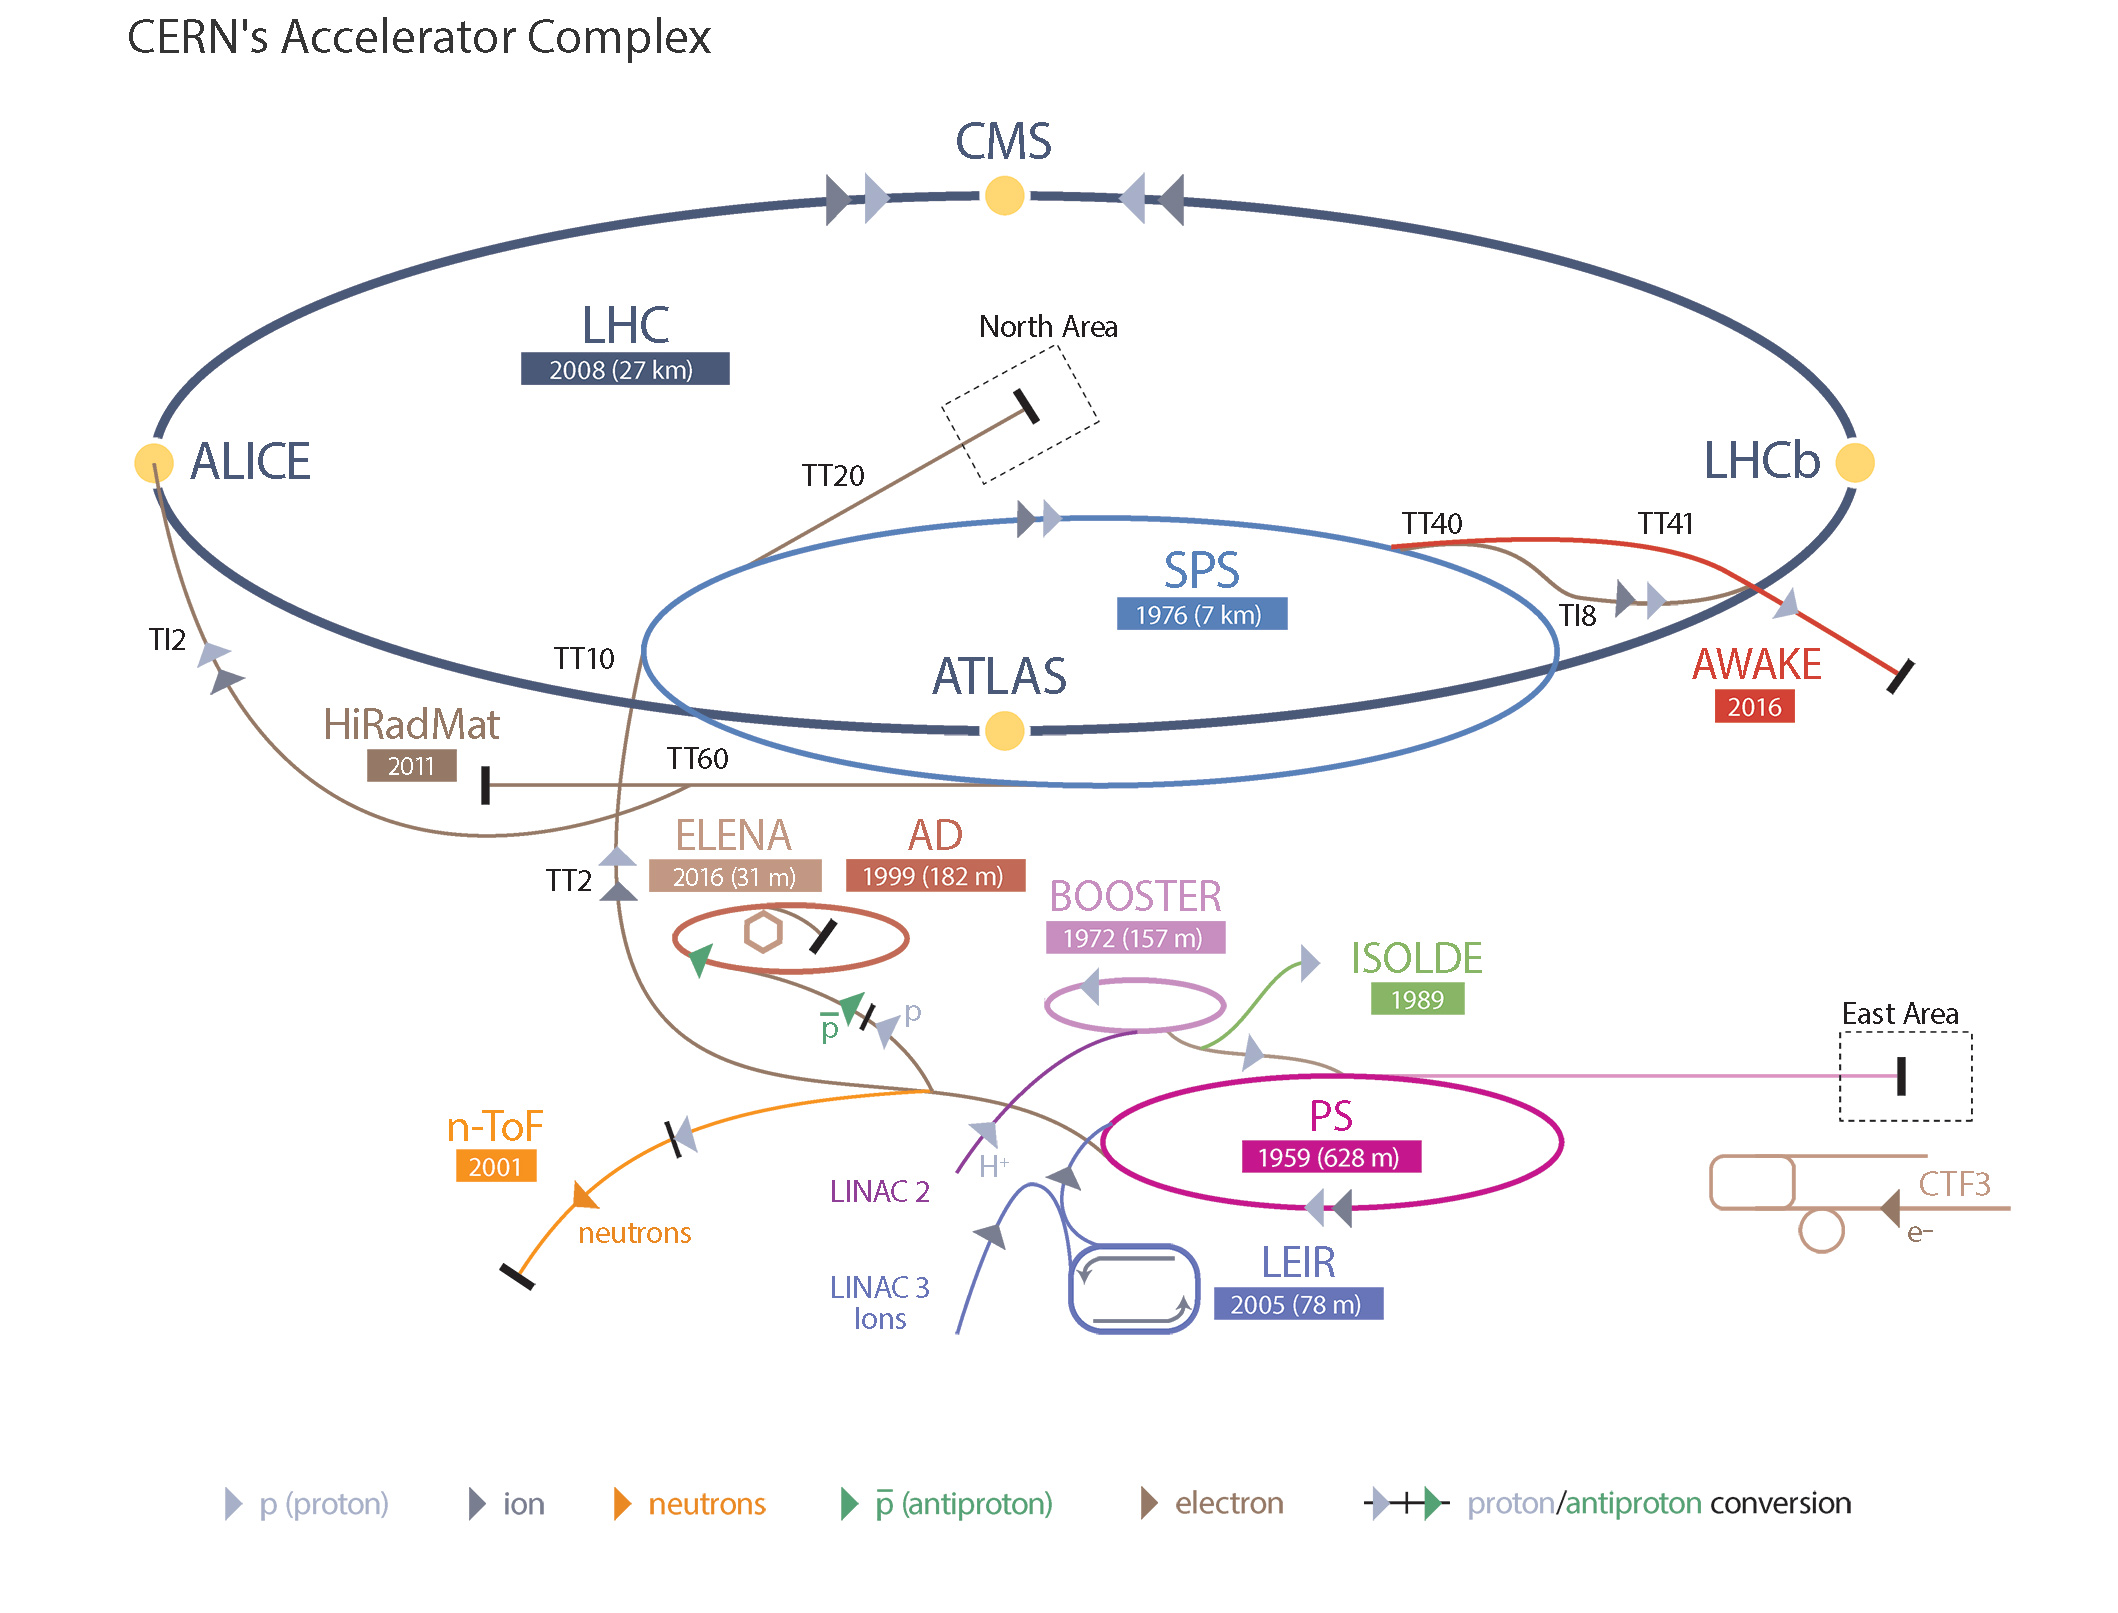
\includegraphics[height=5cm,width=10cm]{2}
\end{frame}

% HHHHHHHHHHHHHHHHHHHHHHHHHHHHHHHHHHHHHHHHHHHHHHHHHHHHHHHHHHHHHHHHH

\begin{frame}[fragile]{The injector chain.}
Before reaching main ring, protons pass by a series of stages:
	\begin{itemize}
		\item Extracted via ionization of Hydrogen in the Duoplasmatron Proton Ion Source.
		\item Accelerated at 50 MeV in Linac2 (1978).
		\item  Linac2 injects protons in the Proton Synchrotron Booster (PSB)
		and are accelerated up to 1.4 GeV.
		\item From PSB, protons are delivered to the Proton Synchrotron (PS) where
		they reach 28 GeV. They are also split from 6 initial bunches to 72, spaced by 25 ns.
		\item  Finally, the pre-acceleration chain is finished by the SPS, the Super Proton Synchrotron. There, the bunches are accelerated up to 450 GeV.
	\end{itemize}
	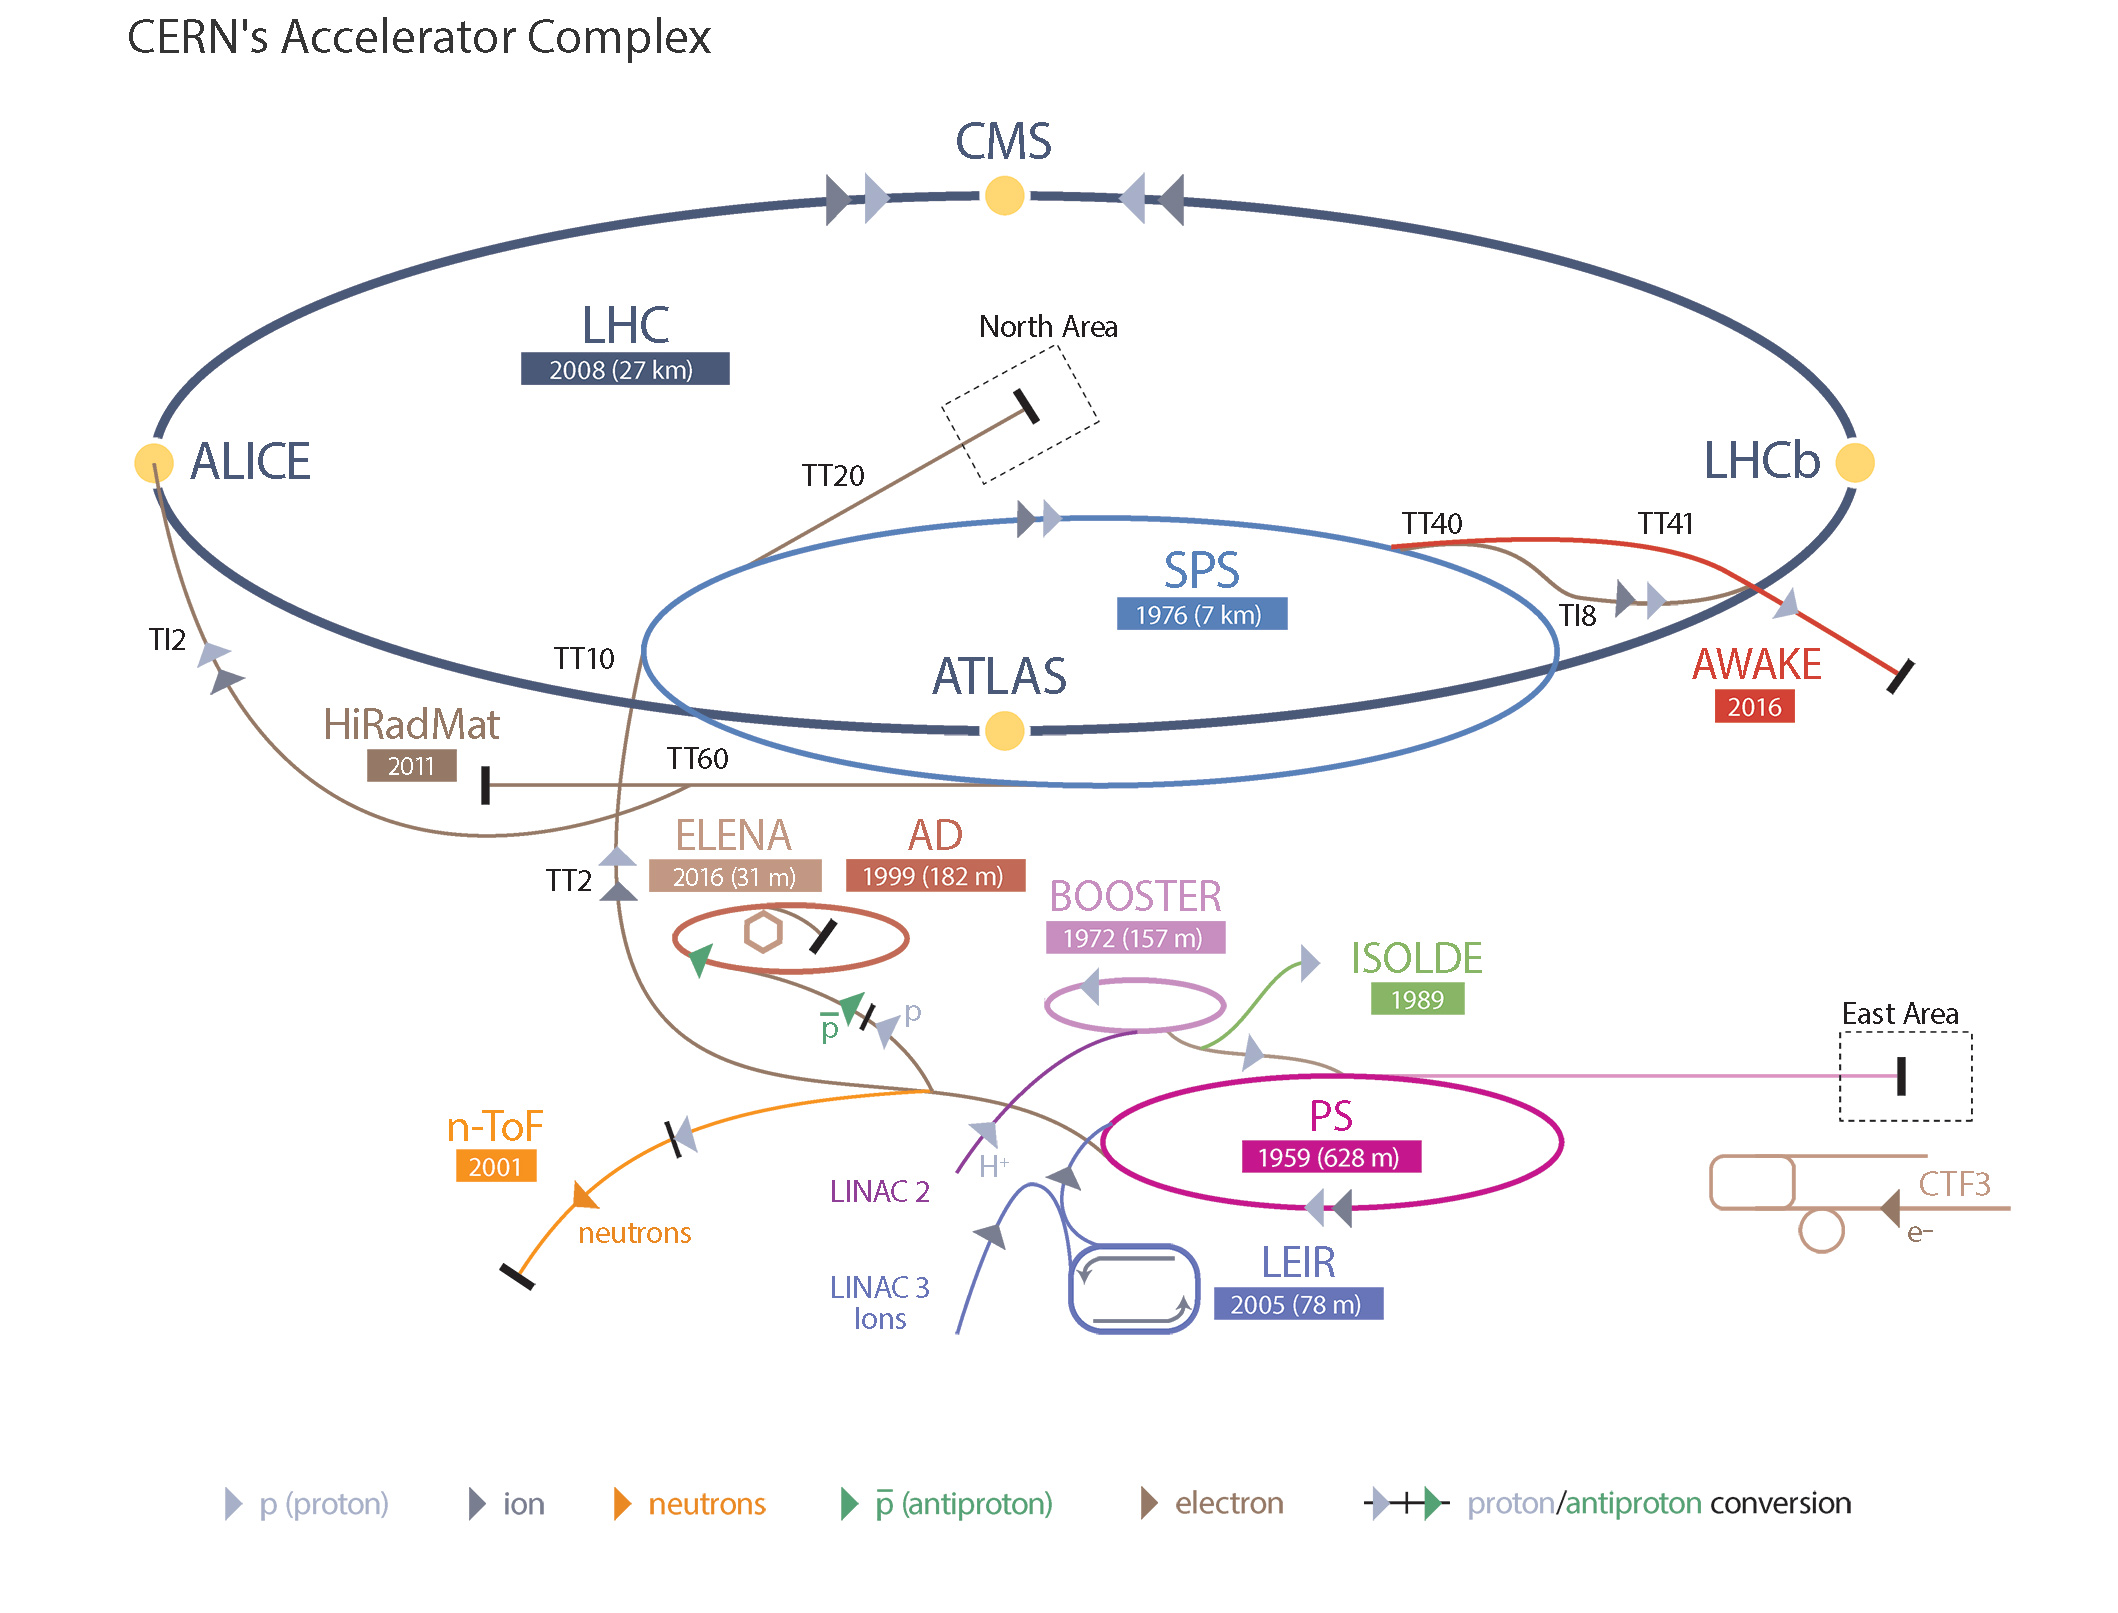
\includegraphics[height=5cm,width=10cm]{2}
\end{frame}

% HHHHHHHHHHHHHHHHHHHHHHHHHHHHHHHHHHHHHHHHHHHHHHHHHHHHHHHHHHHHHHHHH

\begin{frame}[fragile]{LHC main ring.}
	It's composed of two rings that accelerate the proton bunches in opposite directions. Some characteristics of the design are:
	\begin{itemize}
		\item 15m magnets with an strong magnetic field of 8,33T. 
		\item Superconductivity involved (1.9 K).
		\item Ultra high vacuum of $10^{-9}$mbar.
		\item In addition LHC has other magnets to correct different characteristics of the beams: 520 quadrupoles, 2464 sextupoles, 1232 octupoles.
	\end{itemize}
	
	\begin{figure}[!tbp]
		\centering
		\begin{minipage}[b]{0.4\textwidth}
			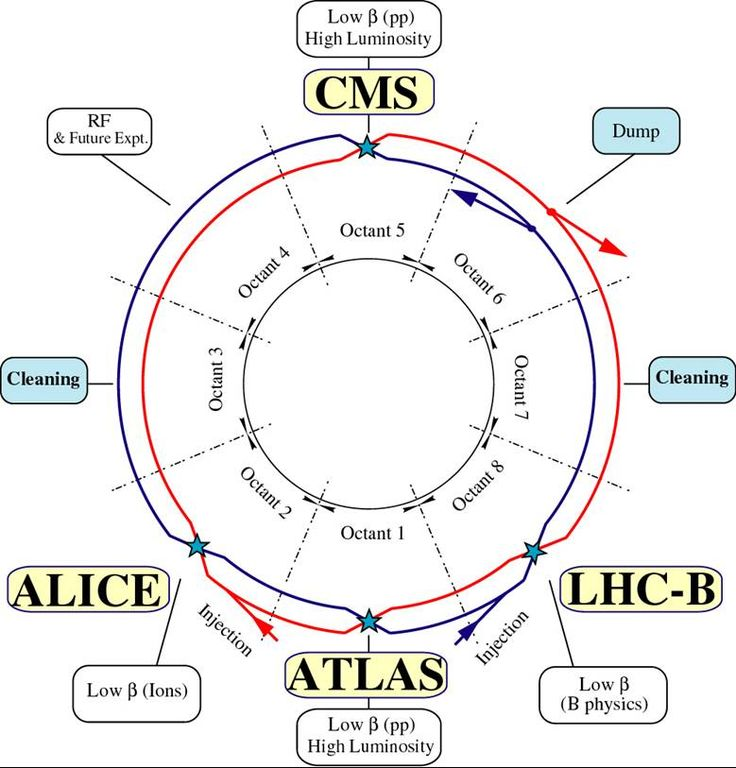
\includegraphics[width=\textwidth]{3}
			
		\end{minipage}
		\hfill
		\begin{minipage}[b]{0.4\textwidth}
			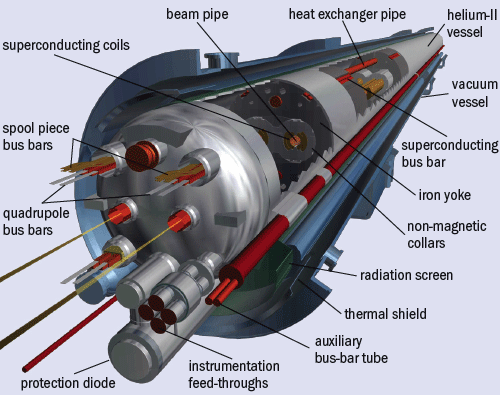
\includegraphics[width=\textwidth]{4}
			
		\end{minipage}
	\end{figure}
\end{frame}

% HHHHHHHHHHHHHHHHHHHHHHHHHHHHHHHHHHHHHHHHHHHHHHHHHHHHHHHHHHHHHHHHH

\begin{frame}[fragile]{LHC main ring.}
	In collider experiments the main character is Luminosity:
\begin{equation}
\nonumber L=\frac{k_nN_{b}^{2}f_{rev}}{4\pi\sigma_x \sigma_y}R
\end{equation}
In LHC design, this parameters have the following values:	
	\begin{table}[]
		\centering
		\label{my-label}
		\begin{tabular}{|l|l|}
			
			\hline
			Energy{[}GeV{]}                                                   &        7000            \\ \hline
			Luminosity{[}$cm^{-2}s^{-1}${]} &      $10^{34}    $           \\ \hline
			$k_b$ Number of bunches                                            &            2808        \\ \hline
			Bunch spacing {[}ns{]}                                            &          24.95          \\ \hline
			$N_b$ intensity per bunch {[}protons/bunch{]}                      &            $1.15\times 10^{11}$        \\ \hline
			$f_{rev}$ revolution frequency {[}kHz{]}                         &           11.25         \\ \hline
			$\sigma_x=\sigma_y$  Beam Standard Deviation  [cm]                    &           7.7         \\ \hline R Geometric reduction factor
			&           0.8         \\ \hline
			
		\end{tabular}
	\end{table}
	Cross section of a proton-proton collision at 14 TeV is 100-110 mb, 3 different processes are involved:
	\begin{itemize}
		\item Elastic scattering: Protons exchange momenta but their structure remains unchanged.
		\item Diffractive scattering: Momenta exchange but additional particles are generated apart from the final protons.
		\item Inelastic scattering: Partons interchange a big amount of momentum and produce several particles.
		
	\end{itemize} 
\end{frame}


% HHHHHHHHHHHHHHHHHHHHHHHHHHHHHHHHHHHHHHHHHHHHHHHHHHHHHHHHHHHHHHHHH

\begin{frame}[fragile]{LHC RUN 1.}
	On February 10th of 2013, the first run of LHC reached an end, this is called RUN 1, started on November 20th of 2009. The achieved center of mass energy was $\sqrt{s}=8TeV$.\\
	\begin{figure}
		\centering
		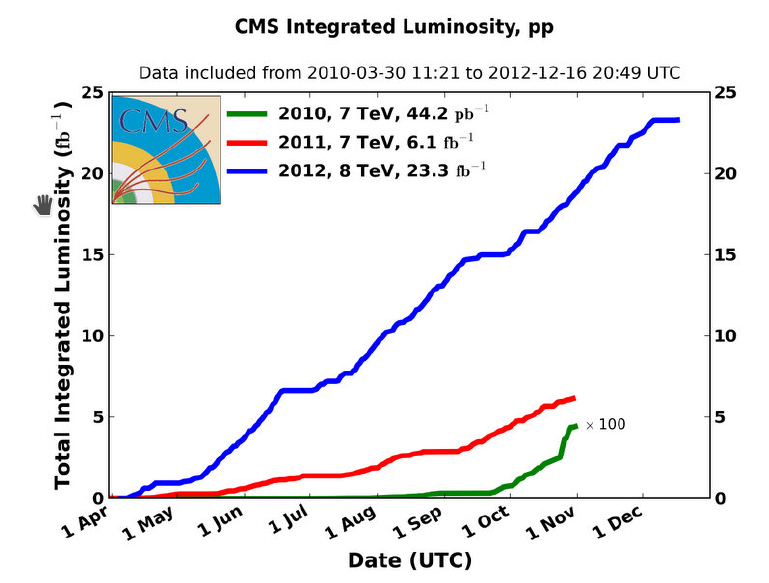
\includegraphics[height=5cm,width=7cm]{5}
		\caption{Integrated Luminosity at LHC RUN 1.}
	\end{figure}	
\end{frame}


% HHHHHHHHHHHHHHHHHHHHHHHHHHHHHHHHHHHHHHHHHHHHHHHHHHHHHHHHHHHHHHHHH

\section{Other experiments at LHC.}

% HHHHHHHHHHHHHHHHHHHHHHHHHHHHHHHHHHHHHHHHHHHHHHHHHHHHHHHHHHHHHHHHH

\begin{frame}[fragile]{ALICE.}
A Large Ion Collider Experiment is located at point 2 of the LHC main ring.

Designed for Heavy Ions Physics.
\\
\begin{minipage}{0.7\textwidth}% adapt widths of minipages to your needs
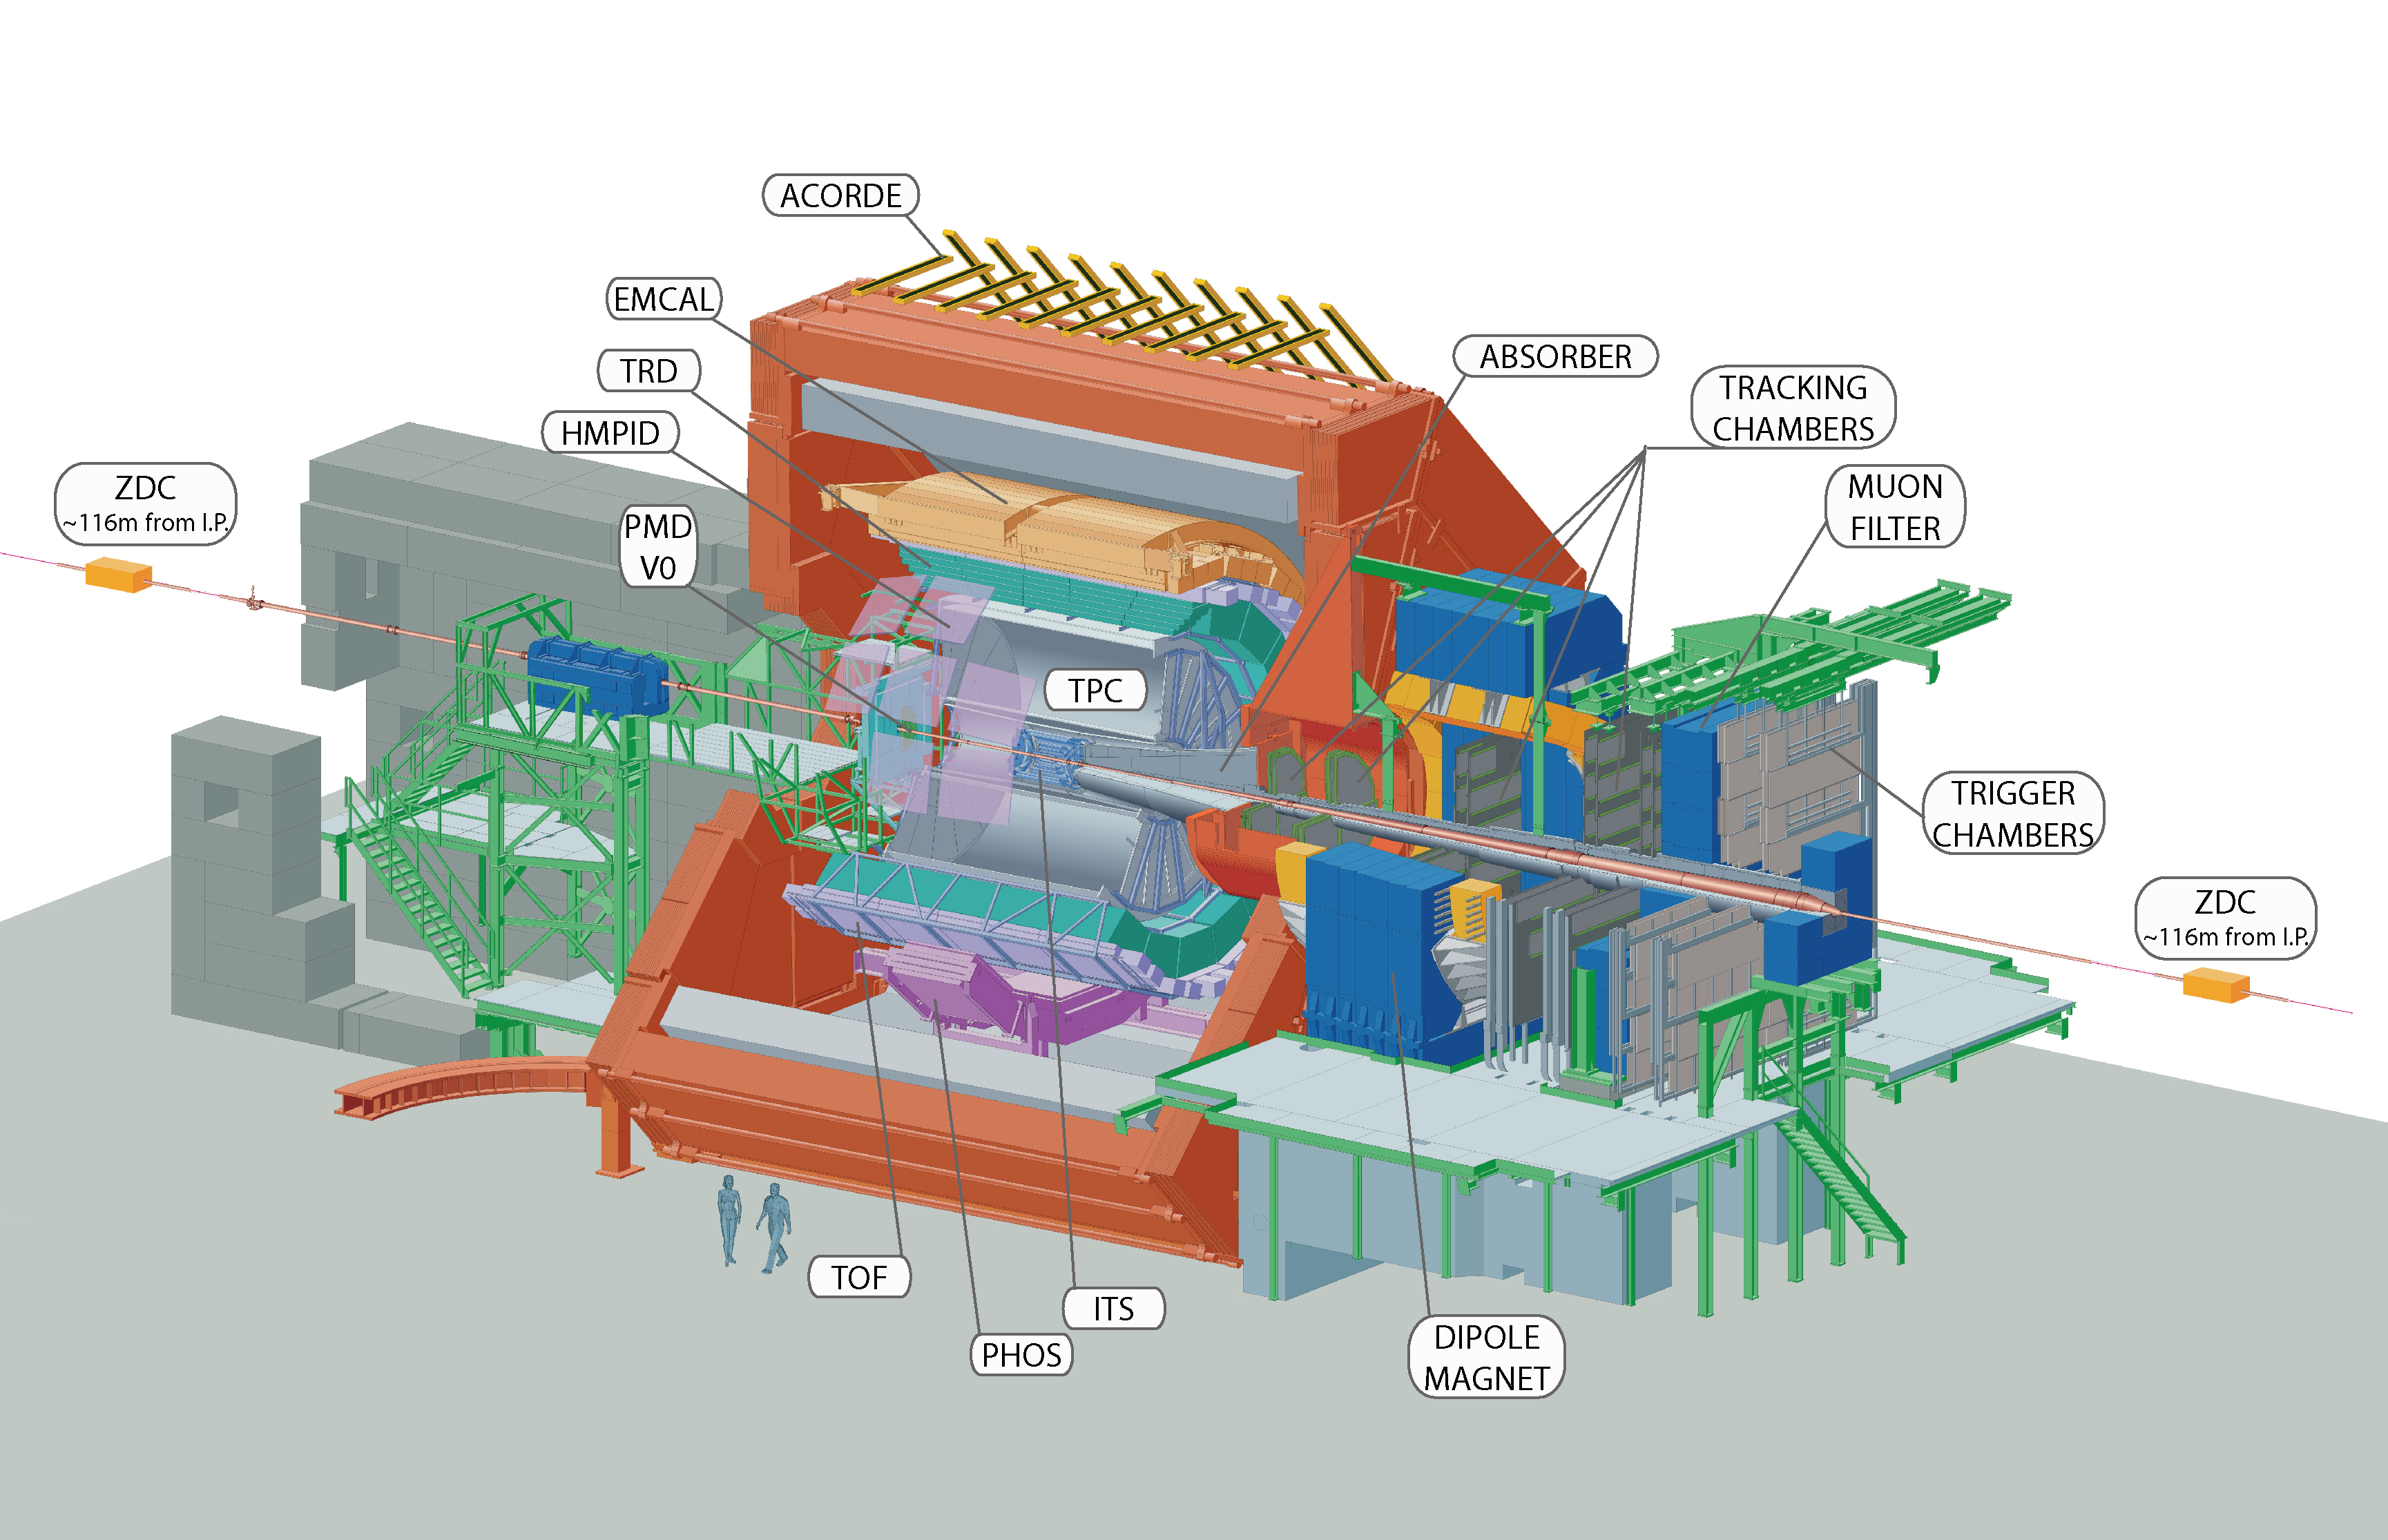
\includegraphics[width=7cm]{6}
\end{minipage}%
\hfill%
\begin{minipage}{0.3\textwidth}\raggedleft
	\begin{itemize}
		\item H=16m,W=16m,L=26m. Weight=10000 Tons.	
		\item Able to detect an extremely high number of tracks per event.
		\item Main subsystem: Time proyection chamber, a 90 $m^3$ gas chamber operated in a soleniod of 0.5T.
	\end{itemize}
\end{minipage}
\\
ALICE collaboration counts around 1500 people from 154 physics institutes in 37 countries.
\end{frame}


\section{CMS.}

\end{document}

